  \documentclass[11pt,a4paper]{article}
\usepackage[utf8]{inputenc}
\usepackage[finnish]{babel}
\usepackage[T1]{fontenc}
\usepackage{amsmath}
\usepackage{amsfonts}
\usepackage{amssymb}
\usepackage{amsthm}
\usepackage{url}
\pagestyle{plain}
\usepackage{graphicx}
\title{Sorbiinihappo}
\author{Delun Li\\014631300\\Orgaanisen kemian työt 1\\Työ 4}
\date{15.10.2018}
\begin{document}

\pagebreak


\maketitle

\pagebreak

\section{Johdanto}

Tässä työssä valmistettiin sorbiinihappoa, \textit{trans}-heksa-2,4-dieenihappoa, malonihaposta ja krotonialdehydistä pyridiinin läsnäollessa. 

\vspace{0.5cm}

\noindent \textbf{Reaktioyhtälö:}$^1$

\vspace{0.3cm}

\hspace{-0.6cm}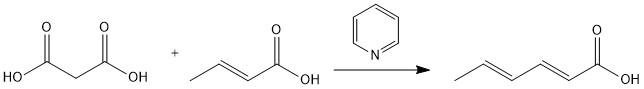
\includegraphics[width=13cm]{sorbiinihappo.jpg}

\vspace{0.5cm}

\noindent \textbf{Reaktio mekanismi:}$^2$

\vspace{0.3cm}

\hspace{-0.6cm}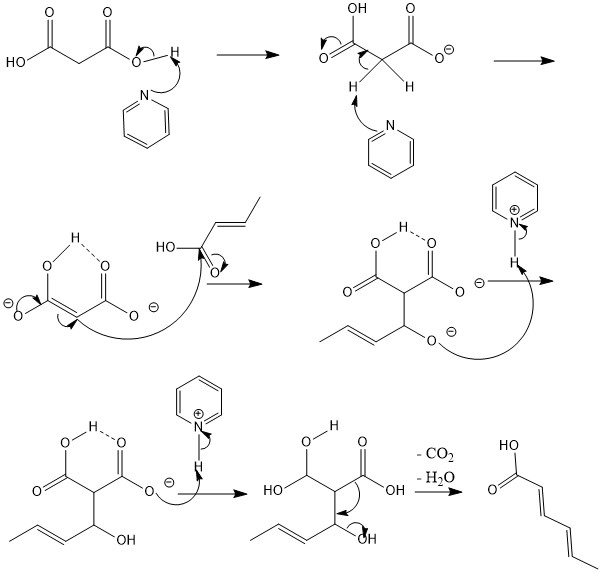
\includegraphics[height=12cm, width=13cm]{sorbiinihappomek.jpg}

\section{Työn suoritus}

Seosta, jossa oli krotonaldehydiä (4,6 ml, 0,0571 mol), malonihappoa (5,96 g , 0,0573 mol) ja pyridiiniä ( 6,1 ml, 0,0759 mol), refluksoitiin kolme tuntia. Kun refluksointi oli loppunut, hapetettiin seosta väkevällä HCl-vesiluoksella (2:5) happamaksi jäähauteessa. Tämän jälkeen seosta jätettiin yön yli jääkaappiin jäähdyttäväksi. 

Jäähtynyt keltainen seos, jossa oli kiinteätä sorbiinihappoa suodatettiin pois ja uudelleenkiteytettiin kiehuvalla vedellä. Uudelleenkiteytyksen jälkeen jätettiin  sorbiinihappo yön yli jääkaappiin ja suodatettiin kiinteä aine. Sorbiinihaposta otettiin saanto (1,846 g, 29$\%$), IR-spektri, $^1$H-NMR ja sulamispiste (133,4 $^\circ$C)

\section{Johtopäätökset}

Tutkimalla liitettä \textbf{IR-spektri}, joka kuvaa sorbiinihapon IR-spektriä, huomataan laaja ja leveä alue 2200-2500 cm$^{-1}$ välillä. Tämä hyvin mahdollisesti esittää karboksyylihapon OH-ryhmän aiheuttamaa venytysvärähtelyä. OH-ryhmän olevan vaihtuvavedyn takia, alue on leveä. Aaltoluvun 2968,52 kohdalla esittää yhdisteen CH$_3$ sp$^3$-sidoksen venytysvärehtelyä. Yhdisteen CH$_2$ sp$^2$-sidosten värähtelyt absorboivat 3020 cm$^{-1}$ tiennoilla. 2500-3000, 1690, 1420, 920 ja 1260 absorptiovyöt johtuvat karboksyyliryhmän olemassaolosta. 1690 kuvaa karboksyyliryhmän C$=$O venytysvärähtelyä, 1260 C-O venytysvärähtelyä ja 1420 ja 920 kuvaavat -OH ryhmän aiheuttamaa taivutusvärähtelyä. $^{3,4}$

Liitteessä \textbf{$^1$H-NMR-spektri}:ssä on esitetty tuotteesta saatu $^1$H-NMR spektri.  Spektristä huomataan, että vetysiirtymät sijoittuvat pitkälti 5,5-7,7 ppm ja 1,5-2,0 ppm välillä. Välillä 5,5-7,7 ppm on useita multiplettia ja 1,75 ppm:n kohdalla on dupletti. Ideaalisessa $^1$H-NMR-spektrissä pitäisi erottua resonanssi n:o 1:llä dupletti, 2:lla dupletti, 3:lla ja 4:llä dupletin dupletti, 5:llä dupletti ja 6:lla singletti. Karboksyylityhmän OH-ryhmän toimii vaihtuvana vetynä, jolloin se sijoittuu 9-13ppm välillä, jota ei näy spektrissä.$^3$  

IR-spektrin, $^1$H-NMR spektrin ja sulamispisteen avulla voidaan sanoa, että tuote on sorbiinihappo. Saatu sorbiinihapon sulamispiste (133,4 $^\circ$C) on hyvin lähellä kirjallisuuden$^5$ (134,5 $^\circ$C). Saanto (29$\%$) on lähellä ohjeen saantoa (31$\%$). Näiden avulla voidaan sanoa, että työ sujui hyvin. 

\pagebreak

\section{Viiteet}
\noindent 1. A.I.Vogel , \textit{Vogel's Textbook of Practical Organic Chemistry}, 4th ed, p.594

\noindent 2. Clayden, \textit{Organic Chemistry}, 2nd ed, s. 630

\noindent 3. Tapio Hase, \textit{Tables For Organic Spectrometry}, \textbf{2008}, s. 20, 30

\noindent 4. \url{https://www.orgchemboulder.com/Spectroscopy/irtutor/carbacidsir.shtml}

\noindent 5. \url{https://pubchem.ncbi.nlm.nih.gov/compound/sorbic_acid#section=Top}

\section{Liiteet}

\noindent $^1$H-NMR-spektri
 
 \noindent $^1$H-NMR : Tulkinta
 
 \noindent IR-spektri
 
 \noindent Synteesikaavake
 
 \noindent Sulamispiste

\end{document}
